\subsection{Opdracht 01}

Geef van een film, de hele reeks waar die bij hoort met volgnummer en in de juiste volgorde.
Indien hij niet in een reeks zit, is de lijst gewoon ��n lang met volgnummer 1.
Dit moet ��n statement worden die van een variabel ID de reeks geeft zoals onderstaand voorbeeld:
DECLARE @MovieInReeks INT = 207989;


\begin{lstlisting}
-- jouw statement hier levert onderstaand resultaat:

ITEM_ID		TITLE				Volgnummer
207992		Matrix, The				1
207989		Matrix Reloaded, The			2
207991		Matrix Revolutions, The		3
\end{lstlisting}

\subsubsection{Versie 01}

    Binnen deze versie is er gebruik gemaakt van een recursieve CTE. Middels een UNION worden de eerste twee SELECT statements
    met elkaar verbonden. Deze vormen de resultset voor het recursieve gedeelte van deze CTE welke zich onder de UNION ALL bevindt.
    Voor de gehele resultset wordt middels de ROW_NUMBER functie het volgnummer van de film bepaald, waarbij de oudste film is voorzien
    van volgnummer 1.

\lstinputlisting[language=SQL]{sql/marc/opdracht-01-01.sql}
\begin{figure}
    \centering
    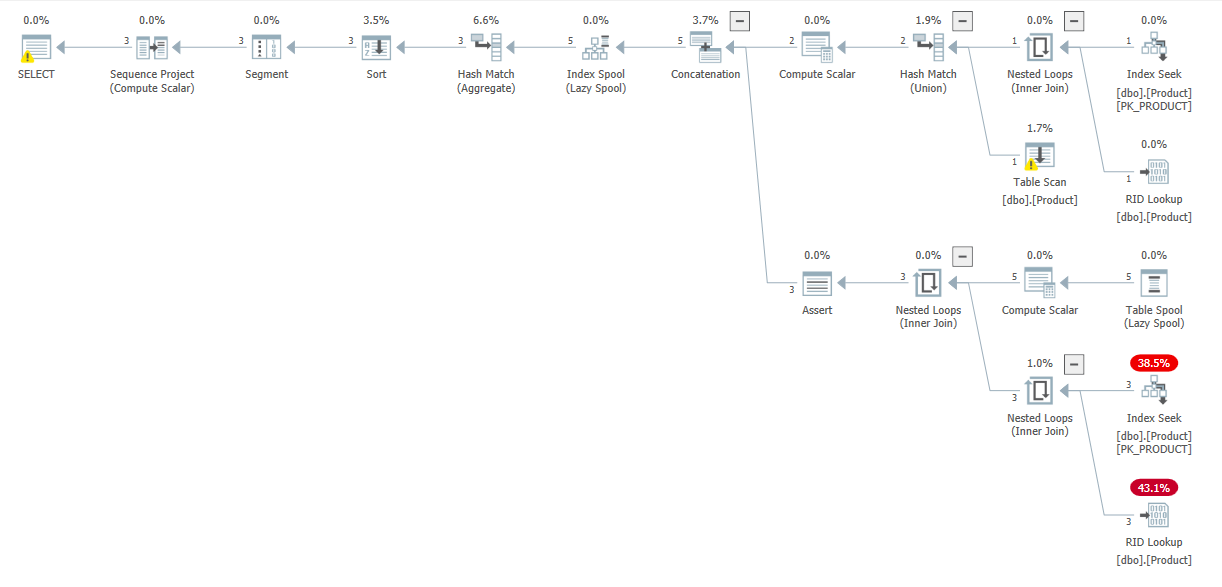
\includegraphics[width=1\textwidth]{image/marc/opdracht-01.PNG}
    \caption{Queryplan Opdracht 01 Versie 01}
\end{figure}

\subsubsection{Versie 02}
TODO: Joey

\lstinputlisting[language=SQL]{sql/joey/opdracht-01-01.sql}
\begin{figure}
    \centering
    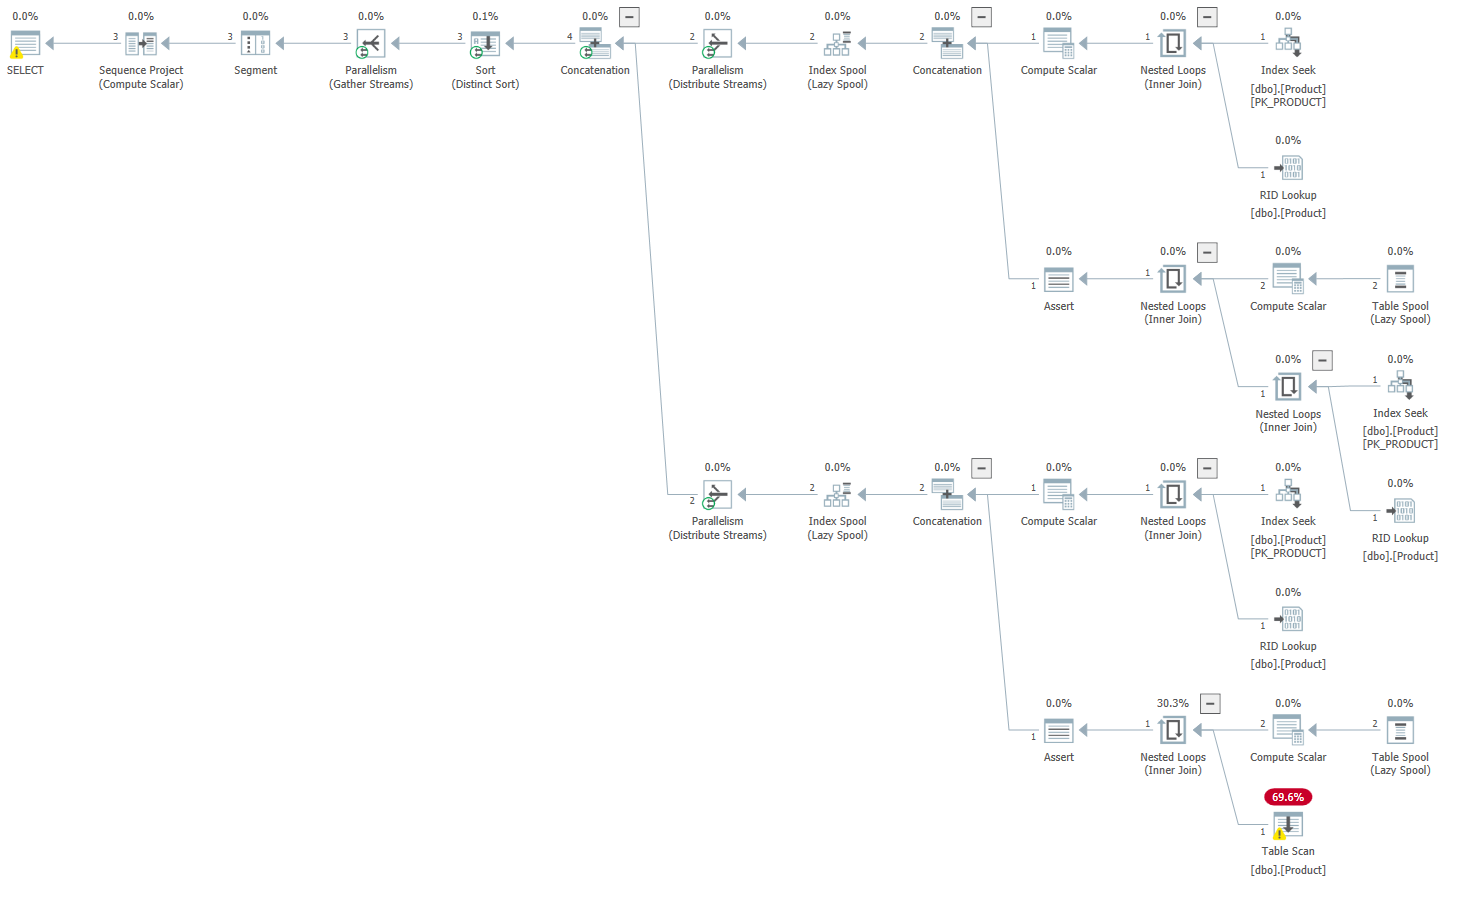
\includegraphics[width=1\textwidth]{image/joey/opdracht-01.PNG}
    \caption{Queryplan Opdracht 01 Versie 02}
\end{figure}


\subsubsection{Versie 03}

    De intentie van deze query was om geen CTE te gebruiken. In dit alternatief maken we gebruik van een tijdelijke tabel.
    Na het aanmaken van van de tijdelijke tabel worden er 2 while loops gedraaid. Bij de eerste loop word er gekeken of er een vorige film is.
    Als die er is, word die opgeslagen in de tijdelijke tabel, en herhaald hij de loop tot het punt komt dat er geen vorige film meer is.
    Hetzelfde doet hij met vervolg films, als deze er zijn word die ook in de tijdelijke tabel opgeslagen.
    Uiteindelijk word de tijdelijke tabel uitgevraagd, en krijg je de lijst met films te zien.
    Als laatste word de tijdelijke tabel verwijderd.

\lstinputlisting[language=SQL]{sql/nick/opdracht-01-01.sql}

\subsubsection{Conclusie}

\begin{tabular}{ || l | l | l | l | l | l | l | l | l | l | l | l | 1 | 1 | l | 1 | 1 || }
    \hline
    \textbf{Statement} & \textbf{Est Cost \%} & \textbf{Compile Time} & \textbf{Duration} &
    \textbf{CPU} & \textbf{Est CPU Cost \%} &
    \textbf{Est IO Cost \%} \\
    \hline
    \hline
    Versie01  & 0,0\%  & 12  & 40  & 40  & 4,9\% & 0,0\% \\
    \hline
    Versie02  & 100,0\%  & 20  & 76  & 75  & 95,1\% & 100,0\%  \\
    \hline
\end{tabular}
\newline
\newline
\begin{tabular}{ || l | l | l | l | l | l | l | l | l | l | l | l | 1 | 1 | l | 1 | 1 || }
    \hline
    \textbf{Statement} &  \textbf{Est Rows} & \textbf{Actual Rows} & \textbf{RID Lookups} &
    \textbf{Parallel} & \textbf{Sort} &
    \textbf{Table Scan} & \textbf{Hash Match} \\
    \hline
    \hline
    Versie01  & 77.765  & 3  & 2  & 0  & 1  & 1  & 2 \\
    \hline
    Versie02  & 1.157.780  & 3  & 3  & 5  & 1  & 1  & 0 \\
    \hline
\end{tabular}


HIer komt dus een lang verhaal over welke query het beste is, en waarom
